\documentclass[12pt, twoside]{article}
\usepackage[letterpaper, margin=1in, headsep=0.5in]{geometry}
\usepackage[english]{babel}
\usepackage[utf8]{inputenc}
\usepackage{amsmath}
\usepackage{amsfonts}
\usepackage{amssymb}
\usepackage{tikz}
\usepackage{yhmath}
%\usetikzlibrary{quotes, angles}

\usepackage{graphicx}
\usepackage{enumitem}
\usepackage{multicol}

\usepackage{fancyhdr}
\pagestyle{fancy}
\fancyhf{}
\renewcommand{\headrulewidth}{0pt} % disable the underline of the header

\fancyhead[RE]{\thepage}
\fancyhead[RO]{\thepage \\ Name: \hspace{3cm}}
\fancyhead[L]{BECA / Dr. Huson / 10th Grade Geometry\\* 3 May 2019}

\begin{document}
\subsubsection*{10.7 Do Now: Volume, density, trig review}
 \begin{enumerate}

   \item $\triangle ABC$ is shown with $m\angle C=90^\circ$ and the lengths of the triangle's sides are $a=5$, $b=8.66$, and $c=10$. \vspace{0.1cm}
     \begin{multicols}{2}
         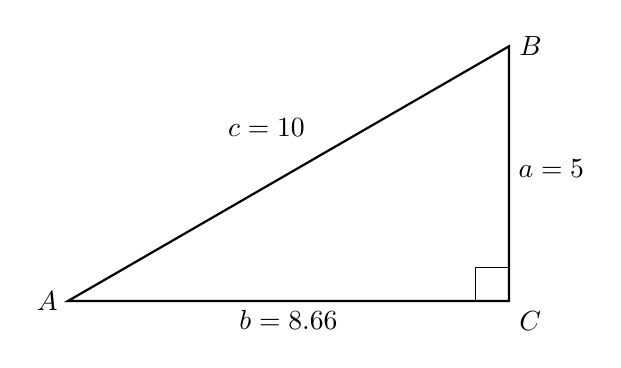
\begin{tikzpicture}[scale=1.4]
           \draw [thick]
           (0,0)node[left]{$A$}--
           (4,0)node[below right]{$C$}--
           (4,2.31)node[right]{$B$}--cycle;
           \draw (4,0)++(-0.3,0)--++(0,0.3)--+(0.3,0);
           \node at (2,0)[below]{$b=8.66$};
           \node at (4,1.2)[right]{$a=5$};
           \node at (1.8,1.4)[above]{$c=10$};
         \end{tikzpicture}

         \begin{enumerate}
         \item Find $\sin A$ \vspace{0.95cm}
         \item Find $\cos A$ \vspace{0.95cm}
         \item Find $\tan A$ \vspace{0.75cm}
       \end{enumerate}
     \end{multicols} \vspace{1.5cm}

   \item Find the area of $\triangle ABC$,  $Area= \frac{1}{2}bh$. The altitude $h$ of the triangle is 18 centimeters and the base $AB=25$ cm.\\[0.5cm]
   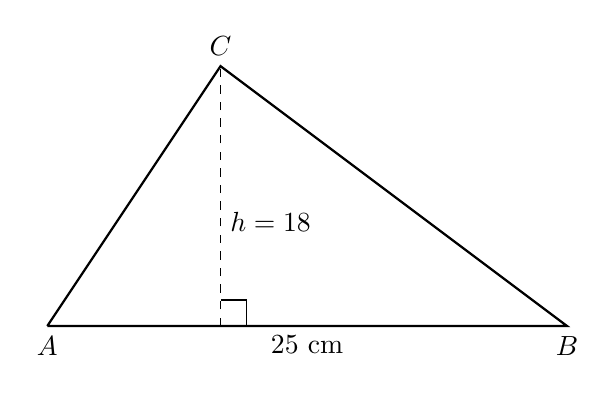
\begin{tikzpicture}[scale=1.1]
     \draw [thick]
       (2,0)node[below]{$A$}--
       (8,0)node[below]{$B$}--
       (4,3)node[above]{$C$} --(2,0);
    \draw [dashed] (4,0)--(4,3);
    \draw (4,0)++(0.3,0)--++(0,0.3)--+(-0.3,0);
    \node at (4,1.2)[right]{$h=18$};
    \node at (5,0)[below]{$25$ cm};
  \end{tikzpicture} \vspace{2.0cm}

   \item Given $S(7,-1)$ and $T(5,3)$, find the length of $\overline{ST}$. Simplify the radical.\vspace{3cm}

\newpage

   \item Find the volume of a cylinder with radius $r=3$ and height $h=10$. Leave your answer in terms of $\pi$ (not a decimal). \vspace{2.5cm}
   \item Find the weight of $60$ liters of gasoline, given that the density of gasoline is $0.73$ kilograms per liter. \vspace{3.0cm}

   \item Circle $O$ has a radius $AO=10$, as shown below, and $m\angle AOB=120^\circ$.
         \begin{center}
         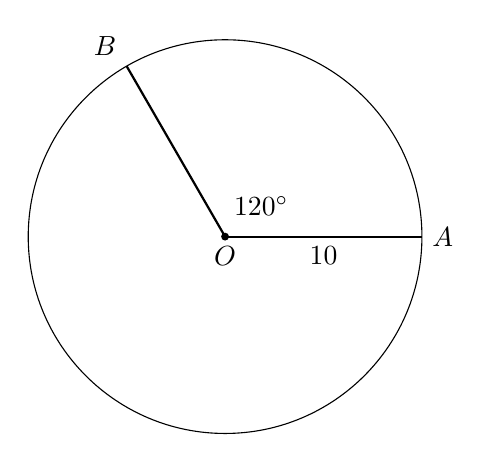
\begin{tikzpicture}[scale=.5]
           \draw (0,0) circle[radius=5];
           \draw [thick]
           (0:5) node[right] {$A$}--(0,0);
           \draw [thick] (0,0)--(120:5) node[above left] {$B$};
           \fill (0,0) circle[radius=0.1] node[below]{$O$};
           \draw (40:1.2) node{$120^\circ$};
           \draw (0:2.5) node[below]{$10$};
           %\draw (75:1.8) node[above] {$C$};
           %\draw (290:5) node[below] {$D$};
         \end{tikzpicture}
       \end{center}
       \begin{enumerate}
         %\item Find the arc measure $m \wideparen{AB}$. \vspace{1.5cm}
         \item Find the length of the arc $\wideparen{AB}$. \vspace{3.5cm}
         \item Find the area of the sector $AOB$. %\vspace{2.5cm}
       \end{enumerate}

  \end{enumerate}
  \newpage
  \setcounter{page}{1}
\subsubsection*{10.7 Classwork: Density, area, \& volume calculations}
 \begin{enumerate}

   \item Express the result to the nearest thousandth.  \vspace{0.5cm}
     \begin{multicols}{2}
       \begin{enumerate}
         \item $\sin 30^\circ = $
         \item $\cos 39^\circ =$
       \end{enumerate}
     \end{multicols} \vspace{0.5cm}

\item Given a circular area $C$ with radius $r=4$ in miles, as shown.

\begin{enumerate}
  \item Find the area of the circle. Round your answer \emph{to the nearest thousandth of a square mile}.\\
    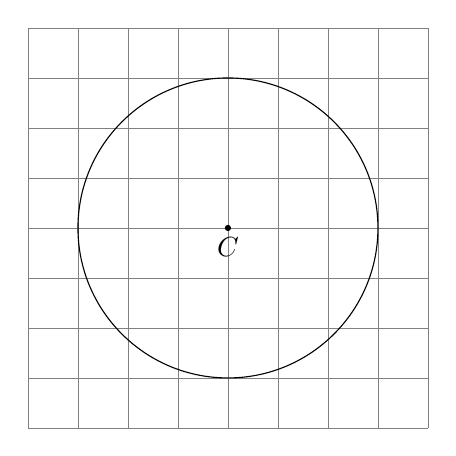
\begin{tikzpicture}[scale=.635]
      \draw [help lines] (-4,-4) grid (4,4);
      %\draw [thick, ->] (-2.2,0) -- (10.4,0) node [below right] {$x$};
      %\draw [thick, ->] (0,-2.2)--(0,10.4) node [left] {$y$};
      \draw (0,0) circle [radius=3] node[below]{$C$};
      \draw [fill] (0,0) circle [radius=0.05];
    \end{tikzpicture}
  \item If each square mile equals $640$ acres, what is the area of the space in acres, \emph{to the nearest acre}?
\end{enumerate} \vspace{2cm}


\item A standard gold bar measures 7 inches long by 3.625 inches wide by 1.75 inches tall.
\begin{enumerate}
  \item Find the volume of the bar in cubic inches (exactly, no rounding). \vspace{2cm}
  \item The density of gold is 0.698 pounds per cubic inch. Find the weight of the bar to the nearest pound.
\end{enumerate}

\newpage

  \item Find the weight of a large glass marble with a diameter of 1.5 inches, to the \emph{nearest tenth of an ounce}. (The formula for the volume of a sphere is $V=\frac{4}{3}\pi r^3$ and the density of glass is 1.49 ounce per cubic inch)  \vspace{9cm}


  \item Find the weight of a stone pyramid ($V=\frac{1}{3}Bh$) having a height of 10 feet and with a square base having side lengths of 12 feet. Express your result to the \emph{nearest pound}. The density of stone is about 150 pounds per cubic foot.


  \end{enumerate}
  \newpage
  \setcounter{page}{1}
\subsubsection*{10.7 Homework: Volume, density, \& trig review}
  \begin{enumerate}

    \item Find the area of a semi-circle radius of 8. Round your answer \emph{to the nearest hundredth}.\vspace{3cm}

    \item Find the volume of a cone ($V=\frac{1}{3}\pi r^2 h$) having a height of 9 inches and with a radius of 4 inches. Express your result to the \emph{nearest cubic inch}. \vspace{7cm}

    \item Find the volume of a cylinder 10 inches tall with a radius of 6 inches, to the \emph{nearest whole cubic inch}. (The formula for the volume of a \emph{cylinder} is $V=\frac{4}{3}\pi r^3$)  \vspace{5cm}

\newpage

    \item Find the area of $\triangle ABC$,  $Area= \frac{1}{2}bh$. The altitude $h$ of the triangle is 29 centimeters and the base $AB=43$ cm.\\[0.5cm]
    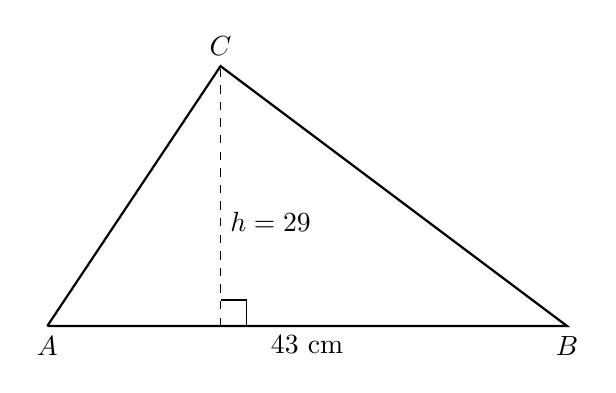
\begin{tikzpicture}[scale=1.1]
      \draw [thick]
        (2,0)node[below]{$A$}--
        (8,0)node[below]{$B$}--
        (4,3)node[above]{$C$} --(2,0);
     \draw [dashed] (4,0)--(4,3);
     \draw (4,0)++(0.3,0)--++(0,0.3)--+(-0.3,0);
     \node at (4,1.2)[right]{$h=29$};
     \node at (5,0)[below]{$43$ cm};
   \end{tikzpicture} \vspace{1.0cm}


   \item Find the weight of a steel ball bearing (sphere) with a radius of 1.0 centimeter, to the \emph{nearest hundredth of a gram}. (The formula for the volume of a sphere is $V=\frac{4}{3}\pi r^3$ and the density of steel is 7.9 grams per cubic cm.)  \vspace{6cm}


   \item Find the weight of a plastic cone ($V=\frac{1}{3}Bh$) having a height of 10 inches and diameter of 12 inches. Express your result to the \emph{nearest ounce}. Use a density of 0.55 ounce per cubic inch for plastic (high density polyethylene).


   \newpage

  \item Express the result to the nearest thousandth.  \vspace{1cm}
    \begin{multicols}{2}
      \begin{enumerate}
        \item $\sin 45^\circ = $ \vspace{1cm}
        \item $\tan 60^\circ =$
        \item $\sin 55^\circ = $ \vspace{1cm}
        \item $\cos 30^\circ =$
      \end{enumerate}
    \end{multicols} %\vspace{0.5cm}

   \item $\triangle ABC$ is shown with $m\angle C=90^\circ$ and the lengths of the triangle's sides are $a=14.14$, $b=10$, and $c=10$. \vspace{0.1cm}
     \begin{multicols}{2}
         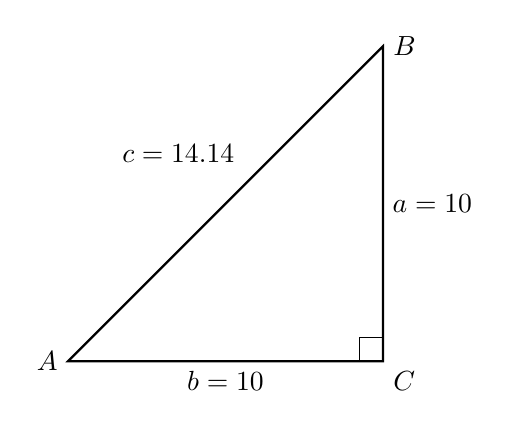
\begin{tikzpicture}[scale=1.0]
           \draw [thick]
           (0,0)node[left]{$A$}--
           (4,0)node[below right]{$C$}--
           (4,4)node[right]{$B$}--cycle;
           \draw (4,0)++(-0.3,0)--++(0,0.3)--+(0.3,0);
           \node at (2,0)[below]{$b=10$};
           \node at (4,2)[right]{$a=10$};
           \node at (1.4,2.4)[above]{$c=14.14$};
         \end{tikzpicture}

         \begin{enumerate}
         \item Find $\sin A$ \vspace{1.25cm}
         \item Find $\cos A$ \vspace{1.25cm}
         \item Find $\tan A$ \vspace{1.cm}
       \end{enumerate}
     \end{multicols} \vspace{1cm}


   \item Given $A(-1,-1)$ and $B(5,2)$, find the length of $\overline{AB}$. Simplify the radical.\vspace{4.cm}

   \item Given $m\angle R=40$ and $m\angle UST=105$. Find $m\angle U$.\\[1cm]
     \begin{tikzpicture}
       %\draw [->, thick] (0,0)--(5,5);
       \draw [<-, thick] (8,0)--(0,0)--(3,3)--(4.5,0);
       \draw [fill] (0,0) circle [radius=0.05] node[below]{$R$};
       \draw [fill] (4.5,0) circle [radius=0.05] node[below]{$S$};
       \draw [fill] (3,3) circle [radius=0.05] node[right]{$U$};
       \draw [fill] (7,0) circle [radius=0.05] node[below]{$T$};
     \end{tikzpicture}
     %\vspace{2cm}

\newpage
\item Given circle $O$ with radius $OB=5.5$.\\[0.5cm]
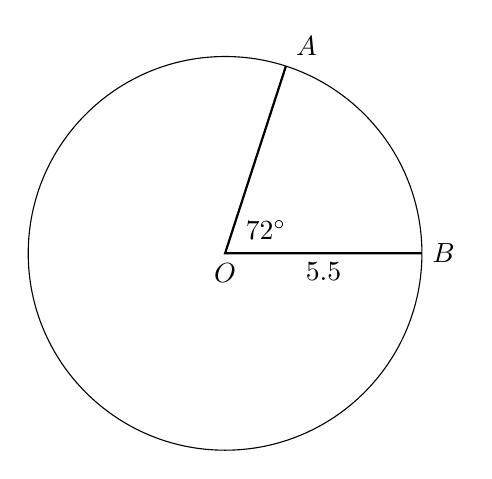
\begin{tikzpicture}[scale=.5]
  \draw (0,0) circle[radius=5];
  \draw [thick]
  (0:5) node[right] {$B$}--
  (0,0) node[below] {$O$}--
  (72:5) node[above right] {$A$};
  \draw (30:1.2) node{$72^\circ$};
  \draw (2.5,0) node[below] {$5.5$};
\end{tikzpicture}
   \begin{enumerate}
     \item Find the circumference of circle $O$. \vspace{2.5cm}
     \item Find its area.  \vspace{4cm}
     \item Given that $m\angle AOB=72^\circ$, find the length of the arc $\wideparen{AB}$. \vspace{3cm}%yhmath package
     \item Find the area of the sector $AOB$. \vspace{1.5cm}
   \end{enumerate}

\end{enumerate}
\end{document}
